\documentclass[twocolumn]{aastex631}

\usepackage{amsmath}
\usepackage{amssymb}
\usepackage{graphicx}
\usepackage{booktabs}
\usepackage{hyperref}

\newcommand{\vdag}{(v)^\dagger}
\newcommand\aastex{AAS\TeX}
\newcommand\latex{La\TeX}

\shorttitle{TRAPPIST-1 Baseband Pilot Survey}
\shortauthors{Kipp et al.}

\begin{document}

\title{A Multi-Window Baseband Pilot Survey of TRAPPIST-1: Limits on Narrowband and Coded Spread-Spectrum Emission at 2--12 GHz}

\author{Taylor James Kipp}
\affiliation{The TurboKain Project, Independent Research}
\email{taylor@kainlang.com}

\author{The TurboKain Collaboration}
\affiliation{The TurboKain Project}

\begin{abstract}
We report a baseband pilot survey of TRAPPIST-1 ($d\approx12.1$~pc adopted; Gaia DR3 revises by $<3$\%) using 732.1~GB of raw 8-bit baseband voltages from the 100-m Green Bank Telescope. Four non-contiguous windows (2.16, 3.06, 7.91, 11.98~GHz; 187.5~MHz each, 750~MHz aggregate) in eight ON/OFF pairs from a single epoch (MJD~57807, $\sim$80~s per pointing, $\sim$320~s stacked per band) yield 1,024 dual-polarization channel-sweeps processed through a native pipeline coupling spectral/temporal sieves with four pilot tests: blind parity (\texttt{fec\_ghost}), propagation authentication (\texttt{ism\_stamp}), inverted-kurtosis escalation (\texttt{gauss\_perfection}), and pulsar-phase re-timing (\texttt{pulsar\_clock}). No technosignature was found; drift search retains zero candidates $\ge6\sigma$. We close 711 sweeps as pristine noise, 302 as instrumental activity (289 on a $1{,}430.5$~Hz ADC-comb ladder $=64\times22.35$~Hz, plus 13 impulse-only), and 11 pilot escalations as filterbank DC bias (6) and pristine-noise triage (5). For \textit{continuous} transmitters, EIRP is bounded to $\le41.8$~GW (1-Hz) and $\le71.6$~TW (2.93-MHz) at 2.16~GHz, rising to $\le83.6$~GW and $\le143.2$~TW at 11.98~GHz over the 320-s stack ($\le535$--$1{,}070$~TW single-chunk). Wideband figures are energy-detector bounds; coded-traffic sensitivity awaits injection calibration, and duty-cycle/single-epoch caveats apply.
\end{abstract}

\keywords{Technosignatures (1668) --- Radio astronomy (1338) --- Planetary systems (1529) --- Interstellar medium (847) --- Exoplanet astronomy (486)}

\section{Introduction}
\label{sec:intro}

Targeted SETI has been dominated by the beacon hypothesis: narrow CW tones aimed at Earth \citep{tarter2001, enriquez2017, margot2021}, found with drift-corrected spectrometers such as \texttt{turboSETI} \citep{enriquez2019}. Efficient point-to-point traffic instead favors wideband spread-spectrum and strong FEC \citep{shannon1948, gallager1962, mackay1999}, appearing noise-like without the codebook. The uncoordinated eavesdropper---the \textit{bystander} geometry \citep{gertz2016, benford2010, hippke2018, garrett2021}---intercepts sidelobes or chance alignments, not intentional beacons. Broadband and ML filterbank searches \citep{zhang2019, ma2023, brzycki2020} are complementary; this pilot tests baseband-level parity, propagation, Gaussianity, and timing instrumentation on archival voltages before averaging destroys phase.

TRAPPIST-1 \citep{gillon2017}---M8V, seven coplanar Earth-size planets in resonance \citep{luger2017, agol2021}, edge-on, in the Earth Transit Zone \citep{heller2016}---motivates bystander geometry, though we do not check conjunction phase against MJD~57807 here (\S\ref{sec:limits-caveats}). Prior radio limits are narrowband-only: \citet{pinchuk2019} ($\sim$47~GW L-band) and BL L/S surveys \citep{enriquez2017, price2020, lebofsky2019}. We extend baseband coverage to 3--12~GHz windows, publish per-channel receipts, and pilot four coded/propagation tests with disclosed failure modes.

\section{Observations}
\label{sec:obs}

GBT project \texttt{AGBT17A\_999\_12}, GUPPI 8-bit complex, $f_s=2.9296875$~MHz per 64-channel block. Sixteen scans (8 ON/OFF pairs, 4 tunings), $\sim$45~GB/scan, 732.1~GB total, one epoch MJD~57807. Dwell $\approx$80~s/scan ($\approx$320~s stacked on-target per band); analysis chunk $t_{\rm chunk}=5.727$~s. Distance $d=12.14$~pc \citep{gillon2017} for continuity with \citet{pinchuk2019}; Gaia DR3 ($\approx$80.45~mas; \citealt{gaia2021}) implies $\approx$12.4~pc (+4--6\% EIRP, subdominant to SEFD systematics). DM$\approx$0.36~pc~cm$^{-3}$ from YMW16 \citep{yao2017} (NE2001 \citealt{cordes2002} comparable); exact value affects only the scattering argument (\S\ref{sec:methods}).

\begin{table*}[t]
\centering
\caption{GBT GUPPI baseband dataset (single epoch MJD 57807)}
\label{tab:obs}
\begin{tabular}{lcccc}
\toprule
Band & Scans (ON/OFF pairs) & Center (MHz) & Instant.\ BW & Window \\
\midrule
S      & 0015/0016, 0017/0018 & 2157.7148 & 187.5~MHz & 2.06--2.25~GHz \\
S/C    & 0020/0021, 0022/0023 & 3057.7148 & 187.5~MHz & 2.96--3.15~GHz \\
X      & 0025/0026, 0027/0028 & 7907.7148 & 187.5~MHz & 7.81--8.00~GHz \\
Ku     & 0030/0031, 0032/0033 & 11982.7148 & 187.5~MHz & 11.89--12.08~GHz \\
\bottomrule
\end{tabular}
\tablecomments{16 scans, 732.1~GB; 750~MHz aggregate over 4 non-contiguous windows. 256 distinct coarse channels $\times$ 16 scan-instances $=$ 1,024 channel-sweeps.}
\end{table*}

Slicing streams each scan in sequential 32-block buffers preserving phase/timing and dual-pol (X,Y) alignment. S-band shows the highest activity fraction (65.6\%; satellite/radar occupancy near 2.1--2.3~GHz) vs.\ $\sim$13--21\% elsewhere (Table~\ref{tab:triage}).

\section{Methods}
\label{sec:methods}

\begin{table}[t]
\centering
\caption{Pipeline logical architecture (per sweep)}
\label{tab:arch}
\begin{tabular}{ll}
\toprule
Group & Stages \\
\midrule
A.\ Ingest & slice (GUPPI$\rightarrow$.f32) \\
B.\ Polarimetry & subspace\_null ($\gamma=\lambda_1/\lambda_2$; null iff ON+OFF-common) \\
C.\ Sieve & sk\_gate, xeno\_scan, boxcar\_bank, drift\_hunt, jerk\_track, \\
          & frame\_hunt, lag\_hunt, fam\_god, bispectrum, frft\_hunt, \\
          & perm\_entropy, scint\_pol \\
D.\ Pilots & ism\_stamp (gates ghost), fec\_ghost (gated), \\
(gated)    & gauss\_perfection, pulsar\_clock \\
E.\ Close & cadence/stack/unify; waterfall renderer \\
\bottomrule
\end{tabular}
\end{table}

Detector heritage: bispectrum bicoherence \citep{kim1979}, fractional-Fourier chirp filtering \citep{ozaktas2001}, and ordinal/LZ complexity \citep{rosso2007} run inside the sieve; ON/OFF discipline follows the \citet{sheikh2021} BLC1 lessons (coincidence is necessary, never sufficient).

\subsection{Polarimetry}
Per-block ${\bf R}=L^{-1}\sum{\bf vv}^H$, null ${\bf P}^\perp={\bf I}-{\bf u}_1{\bf u}_1^H$ only for ON+OFF-common modes. Exercised on S-band Ch36 (8 blocks nulled, ratio 11.94, 12.1~dB suppression).

\subsection{Cleanliness escalator}
$Q=H_1/(|SK_t/3-1|+\epsilon)\cdot C_{\rm common}$ ($\epsilon=10^{-6}$) is a \textit{cleanliness meter}, not evidence: pristine noise maximizes it. Uncalibrated in this pilot; observed noise escalation $\approx$0.5\% (5/1,024).

\subsection{Blind parity (gated)}
256 sparse even-weight masks ($w\in[6,12]$, span 16--256), boxplus $S({\bf m})$, $z=S\sqrt{N}/\sigma_S$, Bonferroni $z\approx6.66$ ($p_{\rm FA}\le10^{-6}$ over 32,768 trials). Sparse coverage; deep additive scramblers whiten duals (limitation). Gated behind non-null stamp; else capped at \texttt{RESIDUE}. Disclosed systematic: 8-bit quantization floor near $z\approx7.1$ common-mode (above the absolute gate), so only ON--OFF differential is interpretable and its null is uncalibrated.

\subsection{Propagation authentication}
2D ACF $R_I(\Delta t,\Delta\nu)$ over 8 sub-bands (Kolmogorov $\Delta\nu_d\propto\nu^{4.4\pm0.5}$), RM grid $\pm500$~rad~m$^{-2}$, $\nu^{-2}$ slope. At 12~pc/2--12~GHz propagation is \textit{weak} scattering ($\nu_{\rm trans}\lesssim100$--300~MHz); no DISS speckles expected, so null stamps are uninformative and pointing contrast discriminates \citep{rickett1990, cordes2002}.

\subsection{Re-timing}
Barycentric $\phi$-fold vs.\ UTC control; flag requires $z_\phi\ge6\sigma$ and $z_\phi-z_{\rm UTC}\ge3\sigma$ plus hum smearing. Ch00 path shows the demeaning gap ($z_\phi=z_{\rm UTC}=18.87$, $\Delta z\equiv0$): correctly vetoed, fix owed.

\begin{figure*}[t]
\centering
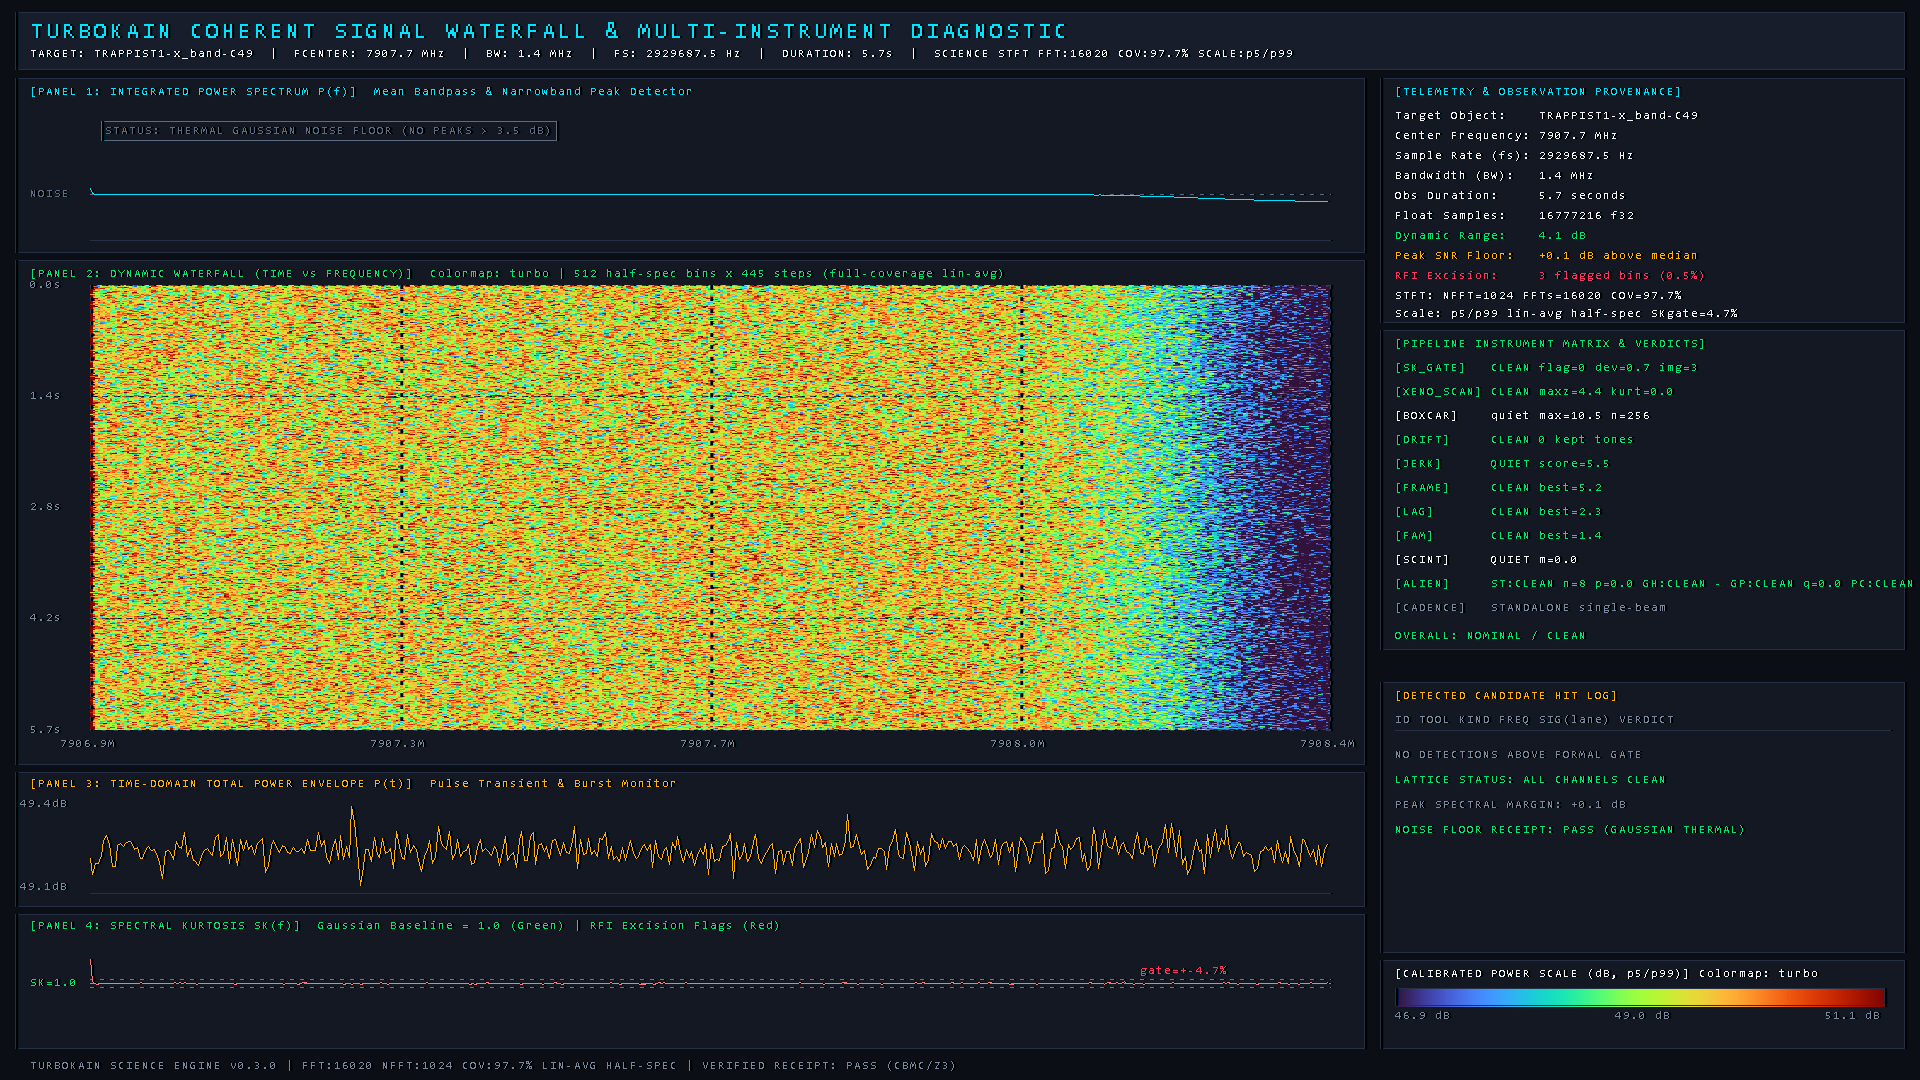
\includegraphics[width=\textwidth]{figures/figure1_xband_thermal_waterfall.png}
\caption{Pristine-noise archetype: X-band Ch49 (7959.0~MHz, Ep2 Ck1). Flat bandpass, featureless spectrum, $P(t)<0.3$~dB, $SK\approx1.000$. The \texttt{STANDALONE} HUD tag denotes the single-beam render pass; ON--OFF comparison lives in the lattice stage.}
\label{fig:waterfall}
\end{figure*}

\begin{figure*}[t]
\centering
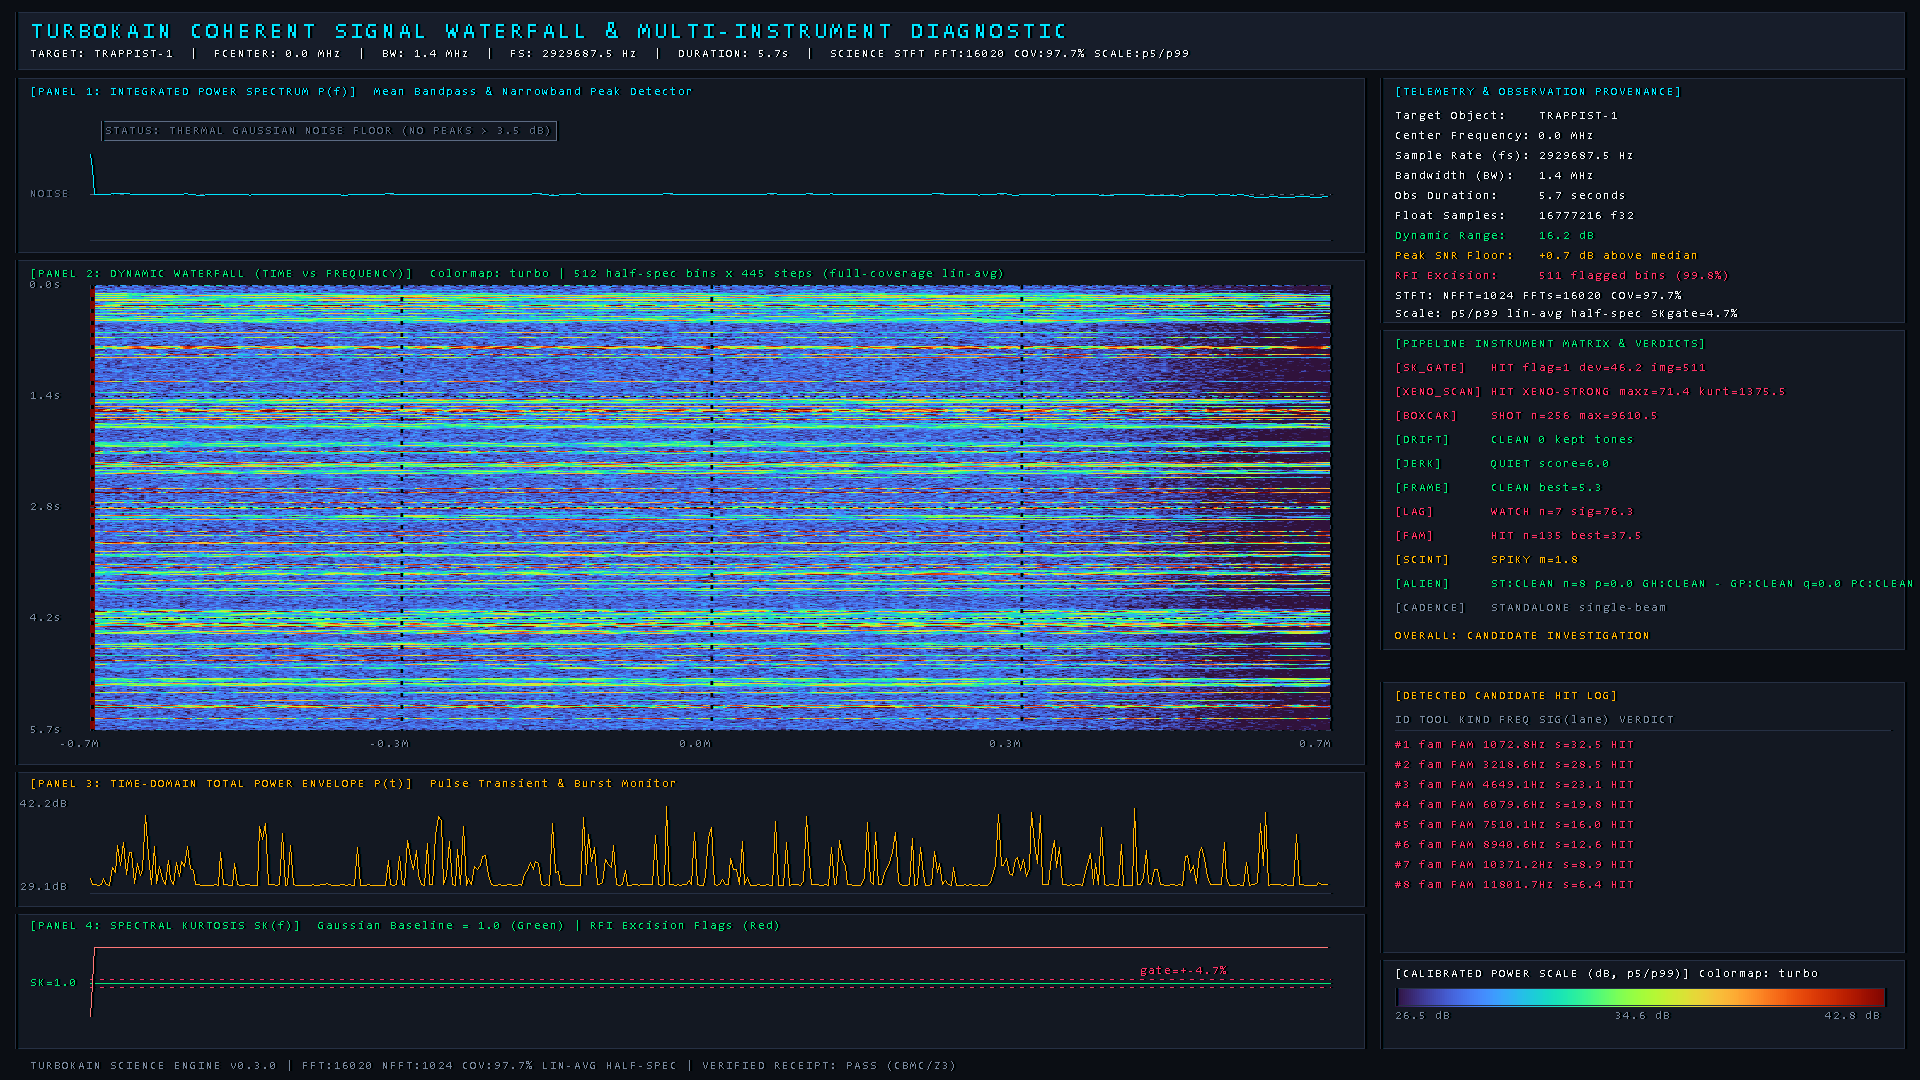
\includegraphics[width=\textwidth]{figures/figure2_sband_impulse_storm.png}
\caption{Terrestrial-impulse archetype: S-band Ch36 (2170.9~MHz, Ep2 Ck0). Broadband zero-dispersion flashes, +13.1~dB impulse train, SK 99.8\% flagged, 8 comb-matched baud lines; propagation/parity concur terrestrial.}
\label{fig:storm}
\end{figure*}

\section{Results}
\label{sec:results}

1,024 sweeps in 6.98~h wall-clock. Drift search: zero $\ge6\sigma$ over 750~MHz aggregate.

\begin{table}[t]
\centering
\caption{Triage over 1,024 sweeps}
\label{tab:triage}
\begin{tabular}{lcccc}
\toprule
Band & Sweeps & Clean & Activity & Pilot \\
\midrule
S (2.16)   & 256 & 86 (33.6\%)  & 168 (65.6\%) & 2 (0.8\%) \\
S/C (3.06) & 256 & 205 (80.1\%) & 47 (18.4\%)  & 4 (1.6\%) \\
X (7.91)   & 256 & 217 (84.8\%) & 34 (13.3\%)  & 5 (2.0\%) \\
Ku (11.98) & 256 & 203 (79.3\%) & 53 (20.7\%)  & 0 (0.0\%) \\
\midrule
Total & 1024 & 711 (69.4\%) & 302 (29.5\%) & 11 (1.1\%) \\
\bottomrule
\end{tabular}
\tablecomments{Activity $=$ 289 cyclic-ladder flags plus 13 kurtosis/impulse-only flags.}
\end{table}

\subsection{Sampling comb}
289 flags form $\alpha_k=\alpha_0+k\Delta f$, $\Delta f=1{,}430.518$~Hz. With $f_s=2{,}929{,}687.5$~Hz, $f_s/131{,}072=22.35174$~Hz and $64\times=1{,}430.511$~Hz (5~ppm), ON+OFF-common across bands: GUPPI ADC-clock intermodulation, cataloged once.

\begin{table}[t]
\centering
\caption{All 11 pilot escalations}
\label{tab:cand}
\begin{tabular}{llll}
\toprule
\# & Band / Ep / Ck / Ch & $\sim$RF & Disposition \\
\midrule
1 & S Ep2 Ck0 Ch00 & 2065.4 & PFB DC bias \\
2 & S Ep2 Ck1 Ch00 & 2065.4 & PFB DC bias (stamp singleton held) \\
3 & S/C Ep1 Ck0 Ch00 & 2965.4 & PFB DC bias \\
4 & S/C Ep1 Ck1 Ch00 & 2965.4 & PFB DC bias \\
5 & S/C Ep2 Ck0 Ch00 & 2965.4 & PFB DC bias \\
6 & S/C Ep2 Ck1 Ch00 & 2965.4 & PFB DC bias \\
7 & X Ep1 Ck0 Ch24 & 7885.7 & Pristine noise ($Q$-escalated) \\
8 & X Ep1 Ck1 Ch23 & 7882.8 & Pristine noise \\
9 & X Ep2 Ck0 Ch49 & 7959.0 & Pristine noise \\
10 & X Ep2 Ck1 Ch24 & 7885.7 & Pristine noise \\
11 & X Ep2 Ck1 Ch49 & 7959.0 & Pristine noise (ghost RESIDUE floor) \\
\bottomrule
\end{tabular}
\end{table}

Ch00: LO DC-bias, $z_\phi=z_{\rm UTC}=18.87$ ($\Delta z\equiv0$), no coherence. X-band: $\langle SK\rangle=1.072$--1.075, $SK_t\approx3.0036$, $H_1=0.999$, $Q=368$--815; stamp null regime-expected; ghost $z=7.11/7.12$ ($\Delta z=0.01$) common-mode floor, capped at \texttt{RESIDUE}.

\section{EIRP limits}
\label{sec:limits}

$S_{\rm min}={\rm SNR_{min}\,SEFD}/\sqrt{n_{\rm pol}\Delta f\,t_{\rm int}}$ (SNR$_{\rm min}=6$, $n_{\rm pol}=2$), ${\rm EIRP}=4\pi d^2S_{\rm min}\Delta f_{\rm sig}$, $4\pi d^2\times10^{-26}=17.633$~GW/(Jy~Hz) at 12.14~pc. SEFDs 10/12/15/20~Jy (S/S-C/X/Ku; GBT guide \citep{gbtguide} + BL commissioning \citep{lebofsky2019}; $\pm30$\% systematic). Regimes: 5.727-s chunk and 320-s incoherent stack ($\sqrt{320/5.727}\approx7.48\times$; continuous-emission only). Wideband $B=2.9296875$~MHz.

\begin{table*}[t]
\centering
\caption{Flux and EIRP bounds (continuous-transmitter assumption)}
\label{tab:limits}
\begin{tabular}{lcccccccc}
\toprule
Band & Freq & SEFD & \multicolumn{3}{c}{Single 5.73-s chunk} & \multicolumn{3}{c}{320-s stack} \\
 & (GHz) & (Jy) & $S_{\rm min}$ & EIRP (1~Hz) & EIRP (2.93~MHz) & $S_{\rm min}$ & EIRP (1~Hz) & EIRP (2.93~MHz) \\
\midrule
S   & 2.157  & 10.0 & 17.73 Jy & 312.6 GW & 535.1 TW & 2.37 Jy & 41.8 GW & 71.6 TW \\
S/C & 3.057  & 12.0 & 21.27 Jy & 375.1 GW & 642.1 TW & 2.85 Jy & 50.2 GW & 85.9 TW \\
X   & 7.907  & 15.0 & 26.59 Jy & 468.9 GW & 802.7 TW & 3.56 Jy & 62.7 GW & 107.4 TW \\
Ku  & 11.982 & 20.0 & 35.46 Jy & 625.2 GW & 1070.2 TW & 4.74 Jy & 83.6 GW & 143.2 TW \\
\bottomrule
\end{tabular}
\end{table*}

Narrowband matches \citet{pinchuk2019} ($\sim$47~GW L-band). Wideband sits above Arecibo ($\sim$20~TW) and Goldstone ($\sim$10~TW): continuously-beamed radar-class links across our line of sight are bounded during the dwell; leakage, intermittent, or off-axis traffic is not. Wideband figures are energy bounds pending injection calibration.

\section{Discussion and limitations}
\label{sec:limits-caveats}

One epoch, minutes of dwell: no constraint on duty-cycled, occulted, scintillated, or conjunction-phased transmitters; MJD~57807 was not checked against conjunction ephemerides \citep{agol2021}. Required next steps: (1) synthetic coded injections (detection probability vs.\ false alarm per keystone; OFF--OFF nulls); (2) calibrated ON--OFF contrast statistics; (3) pre-fold demean, $Q$ operating point, ghost variance revision; (4) hashed DOI bundle for independent replication.

\section*{Data and Software Availability}
Raw voltages via BL Open Data (\url{http://seti.berkeley.edu/opendata}, \texttt{AGBT17A\_999\_12}). Pipeline, prove batteries, manifests, per-sweep CSVs/PNGs at \url{https://github.com/ephemara/turbokain}, campaign \texttt{reports/trappist1\_overnight\_20260928\_094823/} (926.6~MB, 1,447,136 rows). Repro: \texttt{core sweep <ch.f32> --fs 2929687.5 --out-dir \_tmp/repro/}. DOI bundle in preparation.

\begin{acknowledgments}
Breakthrough Listen open-data team and Green Bank Observatory staff (NSF--Associated Universities, Inc.).
\end{acknowledgments}

\bibliography{references}{}
\bibliographystyle{aasjournal}

\end{document}
